\documentclass[11pt,twoside,a4paper]{article}
% http://www-h.eng.cam.ac.uk/help/tpl/textprocessing/latex_maths+pix/node6.html symboles de math
% http://fr.wikibooks.org/wiki/Programmation_LaTeX Programmation latex (wikibook)
%=========================== En-Tete =================================
%--- Insertion de paquetages (optionnel) ---
\usepackage[french]{babel}   % pour dire que le texte est en fran{\'e}ais
\usepackage{a4}	             % pour la taille   
\usepackage[T1]{fontenc}     % pour les font postscript
\usepackage{epsfig}          % pour gerer les images
%\usepackage{psfig}
\usepackage{amsmath, amsthm} % tres bon mode mathematique
\usepackage{amsfonts,amssymb}% permet la definition des ensembles
\usepackage{float}           % pour le placement des figure
\usepackage{verbatim}

\usepackage{longtable} % pour les tableaux de plusieurs pages

\usepackage[table]{xcolor} % couleur de fond des cellules de tableaux

\usepackage{lastpage}

\usepackage{multirow}

\usepackage{multicol} % pour {\'e}crire dans certaines zones en colonnes : \begin{multicols}{nb colonnes}...\end{multicols} 

% \usepackage[top=1.5cm, bottom=1.5cm, left=1.5cm, right=1.5cm]{geometry}
% gauche, haut, droite, bas, entete, ente2txt, pied, txt2pied
\usepackage{vmargin}
\setmarginsrb{0.20cm}{0.20cm}{0.20cm}{0.20cm}{15pt}{3pt}{15pt}{3pt}

\usepackage{lscape} % changement orientation page
%\usepackage{frbib} % enlever pour obtenir references en anglais
% --- style de page (pour les en-tete) ---
\pagestyle{empty}

% % % en-tete et pieds de page configurables : fancyhdr.sty

% http://www.trustonme.net/didactels/250.html

% http://ww3.ac-poitiers.fr/math/tex/pratique/entete/entete.htm
% http://www.ctan.org/tex-archive/macros/latex/contrib/fancyhdr/fancyhdr.pdf
% \usepackage{fancyhdr}
% \pagestyle{fancy}
% % \newcommand{\chaptermark}[1]{\markboth{#1}{}}
% % \newcommand{\sectionmark}[1]{\markright{\thesection\ #1}}
% \fancyhf{}
% \fancyhead[LE,RO]{\bfseries\thepage}
% \fancyhead[LO]{\bfseries\rightmark}
% \fancyhead[RE]{\bfseries\leftmark}
% \fancyfoot[LE]{\thepage /\pageref{LastPage} \hfill
	% TITLE
% \hfill 
\includegraphics[width=0.5cm]{img/logo_glider.png} }
% \fancyfoot[RO]{
\includegraphics[width=0.5cm]{img/logo_glider.png} \hfill
	% TITLE
% \hfill \thepage /\pageref{LastPage}}
% \renewcommand{\headrulewidth}{0.5pt}
% \renewcommand{\footrulewidth}{0.5pt}
% \addtolength{\headheight}{0.5pt}
% \fancypagestyle{plain}{
	% \fancyhead{}
	% \renewcommand{\headrulewidth}{0pt}
% }


%============================= Corps =================================
\begin{document}

\setlength\parindent{0pt}

\texttt{http://ploum.net/post/208-le-plus-grand-jeu-en-ligne-massivement-multi-joueurs-du-monde}~\\

\textbf{\LARGE Le plus grand jeu en ligne massivement multi-joueurs du monde}

\emph{\small Le samedi, mars 14 2009, 18:18 :: advocacy, best seller, planetlibre}

\begin{minipage}[ht]{6.5cm}
	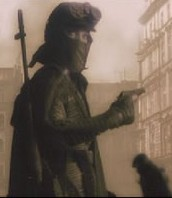
\includegraphics[width=6.45cm]{img/avalon.jpg}
\end{minipage} \hfill \begin{minipage}[ht]{0.65\textwidth}
	L'une des critiques que j'entends le plus r{\'e}guli{\`e}rement {\`a} propos de l'utilisation de Linux est le manque de jeux pour cette plate-forme. L{\`a}, je corrige tout de suite, des jeux il y en a, et des centaines. Il suffit de lire le \textbf{blog de Yekcim~\footnote{\texttt{http://yeknan.free.fr/dc2/index.php?tag/jeux}}} pour s'en convaincre. Depuis le \textbf{FPS galactique~\footnote{\texttt{http://tremulous.net/}}} au  \textbf{counterstrike-like~\footnote{\texttt{http://www.tcelite.net/}}} en passant par les \textbf{petites perles~\footnote{\texttt{http://2dboy.com/games.php}}}.

	L{\`a}, je vous vois venir : oui mais il manque un vrai grand jeu. Une {\'e}pop{\'e}e massivement multijoueurs, un univers virtuel o{\`u} s'immerger. Un jeu o{\`u} incarner un gourou magicien qui sauve le monde avec l'aide de sa guilde, un jeu o{\`u} le temps pass{\'e} permet d'acqu{\'e}rir de l'exp{\'e}rience, des supers pouvoirs. Un jeu o{\`u} les meilleurs sont reconnus par leurs pairs, une seconde vie virtuelle {\`a} propos de laquelle on peut discuter sur les fora o{\`u} dans les cours de r{\'e}cr{\'e}. Ce genre de jeu n'existe pas pour Linux.~\\
\end{minipage}~\\~\\

\begin{minipage}[ht]{0.30\textwidth}
	Quoi ? Ce genre de jeu n'existe pas pour Linux ?~\\
	Vous voulez passer des heures {\`a} apprendre, {\`a} vous entra{\^i}ner pour augmenter votre niveau d'exp{\'e}rience ? Vous voulez faire partie d'un groupe rassembl{\'e} autour d'une qu{\^e}te commune ? Vous voulez faire vivre votre avatar dans le plus grand univers virtuel qui soit ? Vous voulez trembler d'inqui{\'e}tude certains jours et faire la f{\^e}te le lendemain suite {\`a} une bonne nouvelle ?~\\
\end{minipage} \hfill \begin{minipage}[ht]{14.10cm}
	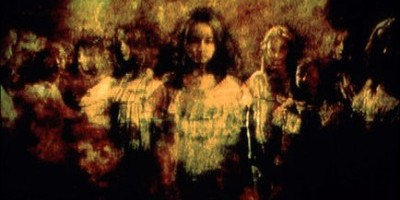
\includegraphics[width=14.05cm]{img/avalon_sisters.jpg}
\end{minipage}~\\~\\

J'ai ce qu'il vous faut. L'histoire est classique : une grande multinationale {\`a} le contr{\^o}le d'une majorit{\'e} des moyens de communication et des ordinateurs de la plan{\`e}te. Cette multi-nationale est m{\^e}me soutenue par la plupart des gouvernements et par les hommes les plus riches du monde. Les citoyens, sous le contr{\^o}le de cette multi-nationale, subissent chaque jour les avanies de cette situation sans en {\^e}tre vraiment conscients et en l'acceptant avec fatalit{\'e}.~\\

\begin{minipage}[ht]{14.10cm}
	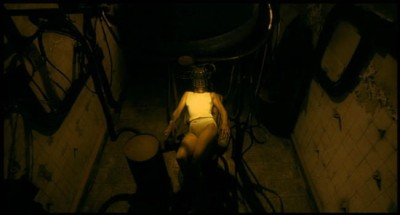
\includegraphics[width=14.05cm]{img/avalon_game.jpg}
\end{minipage} \hfill \begin{minipage}[ht]{0.30\textwidth}
	Vous fa{\^i}tes partie d'un groupe qui a pris conscience de cet {\'e}tat de fait. Vous refusez {\`a} vous r{\'e}signer et {\`a} abandonner votre choix personnel et votre libert{\'e}. Pour sauvegarder cette libert{\'e} si pr{\'e}cieuse, il va falloir lutter. Chaque jour, chaque instant est sera un combat contre l'empire d'une multi-nationale, contre la passivit{\'e} de votre entourage, contre les pr{\'e}jug{\'e}s.~\\
\end{minipage}~\\

\vfill
\clearpage
\vfill

Tout comme le premier grec au sommet de l'Olympe {\`a} son retour {\`a} Ath{\`e}nes~\footnote{Je n'arrive pas {\`a} retrouver le nom ni l'histoire exacte de ce grec qui, arriv{\'e} au sommet de l'Olympe, ne vit rien de sp{\'e}cial et redescendit pour annoncer au peuple que les dieux n'existaient pas. Il f{\^u}t trait{\'e} de menteur et mis {\`a} mort. L'histoire nous est racont{\'e}e par un philosophe grec mais je n'arrive plus {\`a} mettre la main dessus. Toute ma reconnaince au premier {\`a} m'envoyer l'histoire. \emph{Bellerophon} }, vous d{\'e}couvrirez que vos pires ennemis sont vos anciens compagnons de captivit{\'e}, \textbf{effray{\'e}s~\footnote{\texttt {http://ploum.net/post/197-le-conte-du-mousse-et-des-vingt-neuf-navires}}} par l'id{\'e}e d'une libert{\'e} qu'ils n'ont jamais connue.~\\~\\~\\

\begin{minipage}[ht]{0.30\textwidth}
	Bienvenue dans le plus grand jeu en ligne massivement multi-joueurs, bienvenue sous Linux !
\end{minipage} \hfill \begin{minipage}[ht]{14.10cm}
	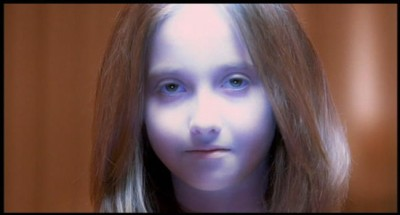
\includegraphics[width=14.05cm]{img/avalon27.jpg}
\end{minipage}~\\~\\~\\

Au d{\'e}but, il vous faudra lutter pour acqu{\'e}rir cette \textbf{fameuse libert{\'e}~\footnote{\texttt{http://ploum.net/post/62-de-la-liberte-la-face-meconnue-de-l-informatique}}}. Apprendre un nouveau syst{\`e}me, de nouveaux logiciels, apprendre {\`a} se d{\'e}brouiller face {\`a} l'adversit{\'e}. Une contribution toute simple, {\`a} la port{\'e}e de tous les joueurs : d{\^i}tes tout haut que vous utilisez Linux. Pas besoin de discours, pas besoin de technique. Vous croyez n'avoir aucun effet mais votre petite affirmation rentrera petit {\`a} petit dans l'inconscience populaire. La prochaine fois que le mot "Linux" appara{\^i}tra, ce ne sera plus une inconnue, cela sera "Ah oui, j'ai entendu parler de ce truc". La premi{\`e}re {\'e}tape : l'acceptation qu'il puisse exister autre chose. L'ouverture {\`a} la diff{\'e}rence. ~\\~\\~\\

\begin{minipage}[ht]{14.10cm}
	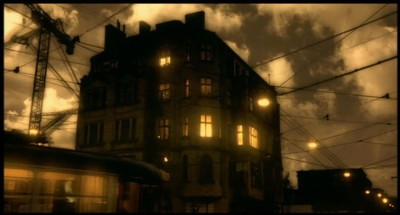
\includegraphics[width=14.05cm]{img/avalon10.jpg}
\end{minipage} \hfill \begin{minipage}[ht]{0.30\textwidth}
	Vous pouvez choisir d'en rester l{\`a} et c'est tr{\`e}s bien. Mais si vous {\^e}tre pris dans l'engrenage, vous risquez tr{\`e}s vite de devenir accro : aide des d{\'e}butants, contributions aux traductions, {\`a} la documentation. Vous commencerez {\`a} vous familiariser avec votre nouvel univers : ligne de commande, entraide, ergonomie... ~\\
\end{minipage}~\\

\vfill
\clearpage
\vfill

\begin{minipage}[ht]{0.30\textwidth}
	Certains en arriveront {\`a} ouvrir un blog, {\`a} aider les programmeurs {\`a} g{\'e}rer les rapports de bugs. Finalement, vous vous retrouverez peut-{\^e}tre m{\^e}me {\`a} coder ou contribuer artistiquement {\`a} des projets pour les am{\'e}liorer. En les am{\'e}liorant, vous les rendez encore plus attractifs aux yeux des nouveaux venus, devenant un "gourou" voire un "hacker", honneur supr{\^e}me.
\end{minipage} \hfill \begin{minipage}[ht]{14.10cm}
	
\includegraphics[width=14.05cm]{img/avalon_window.jpg}
\end{minipage}~\\~\\~\\

Si vous choisissez la classe "pros{\'e}lyte", votre exp{\'e}rience vous permettra de convaincre votre entourage sans avoir l'air d'un gros boulet monomaniaque. Vous acquerrez petit {\`a} petit la diplomatie, l'empathie et l'art de la manipulation. Vos auditeurs deviendront eux aussi des joueurs qui grossiront les rangs de votre guilde.~\\~\\~\\

\begin{minipage}[ht]{14.10cm}
	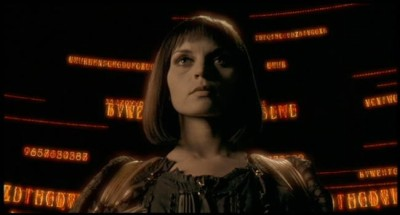
\includegraphics[width=14.05cm]{img/avalon_final.jpg}
\end{minipage} \hfill \begin{minipage}[ht]{0.30\textwidth}
	Pas de jeu sous Linux ? Laissez moi rire, Linux est le plus grand jeu du monde ! Un jeu qui se construit par les joueurs eux-m{\^e}mes, un monde {\`a} la fronti{\`e}re entre le virtuel et le r{\'e}el.~\\
	Et, {\`a} ma connaissance, il s'agit du seul jeu au monde dont vous pouvez vous vanter sur votre CV d'y passer des nuits blanches.~\\

	\textbf{Level complete...}~\\

	\textbf{Bienvenue sous Linux...}~\\
\end{minipage}~\\

\end{document}
